\chapter{Le Kerala de Munnar à Kovalam}
\section*{15 novembre 2015}
Longue descente et quelques cols pour revenir sur la côte, il m'arrive de faire quelques dizaines de km sans croiser personne, c'est rare en Inde ! \newline
 \newline
\centerline{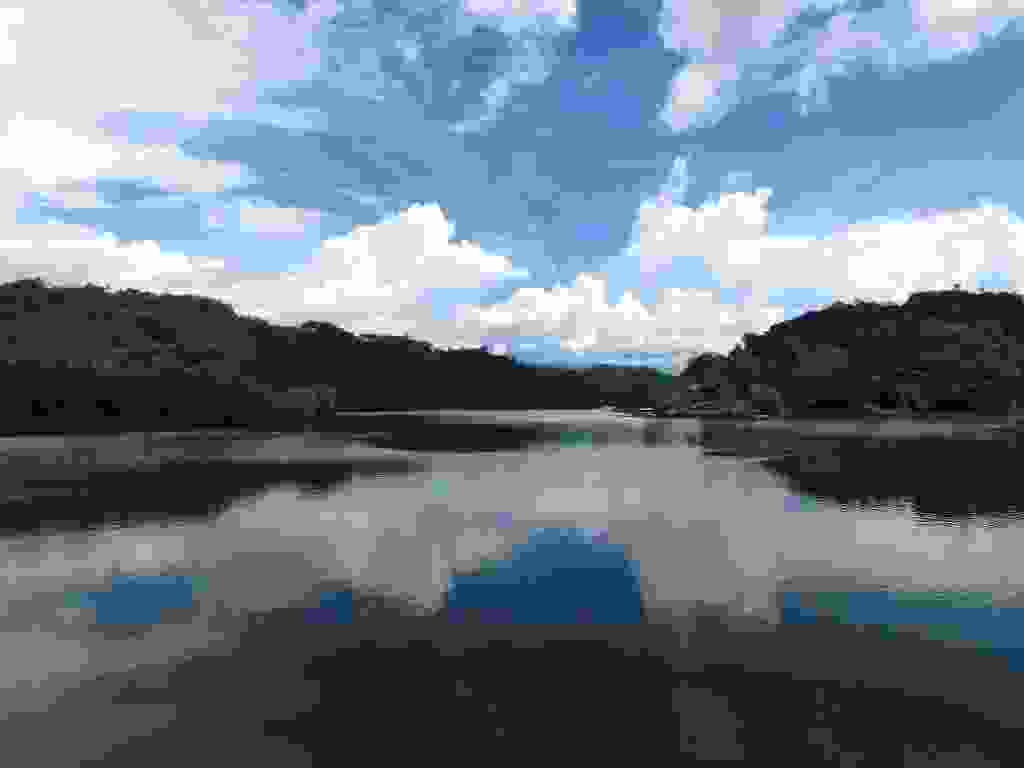
\includegraphics[width=\mywidth]{../wp-content/uploads/2015/11/wpid-oi0001863-1024x768.jpg} } 
 \newline
 \newline
\centerline{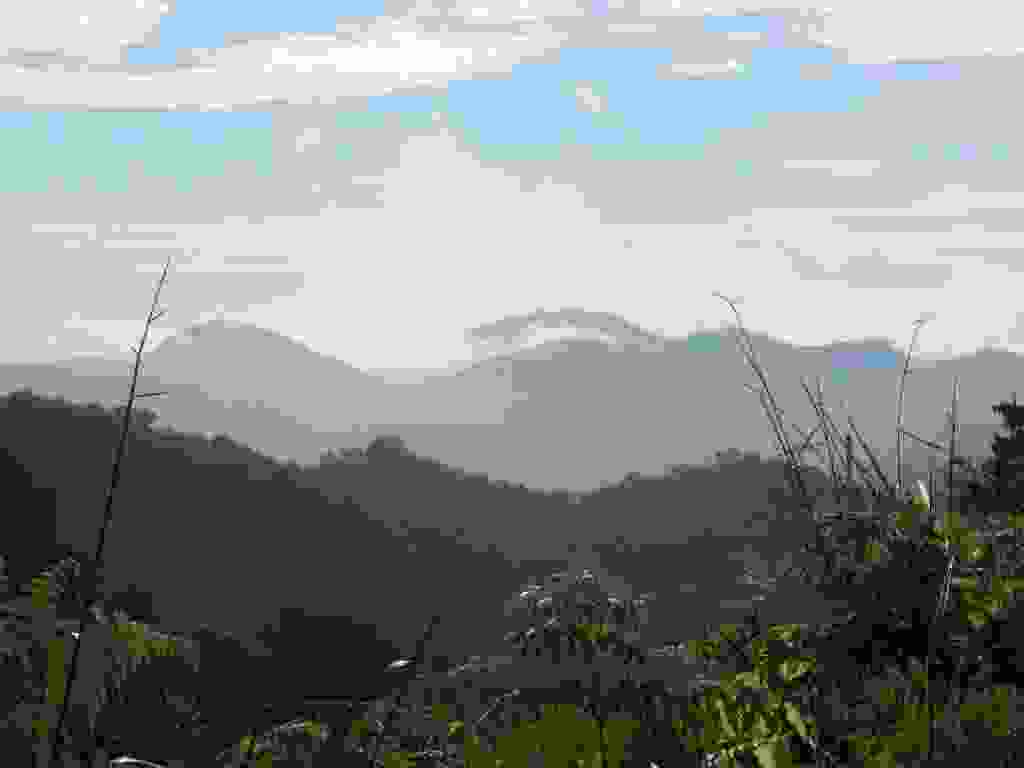
\includegraphics[width=\mywidth]{../wp-content/uploads/2015/11/wpid-oi0002643-1024x768.jpg} } 
 \newline
 \newline
\centerline{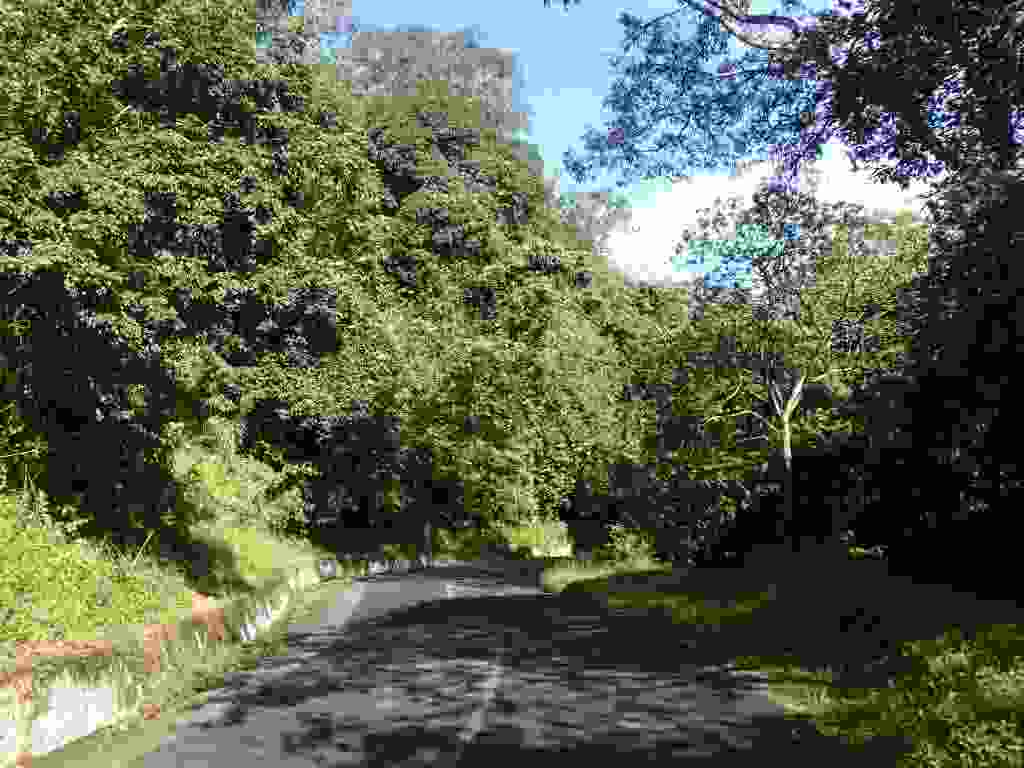
\includegraphics[width=\mywidth]{../wp-content/uploads/2015/11/wpid-oi0002653-1024x768.jpg} } 
 \newline
 \newline
\centerline{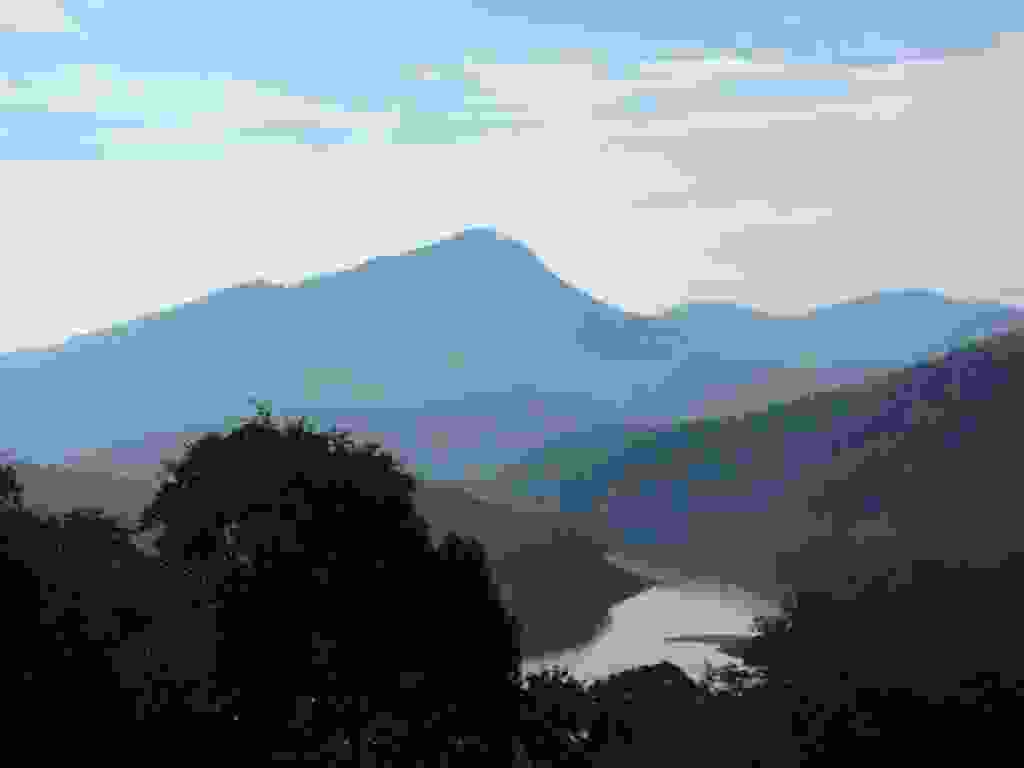
\includegraphics[width=\mywidth]{../wp-content/uploads/2015/11/wpid-oi0002672-1024x768.jpg} } 
 \newline
 \newline
\centerline{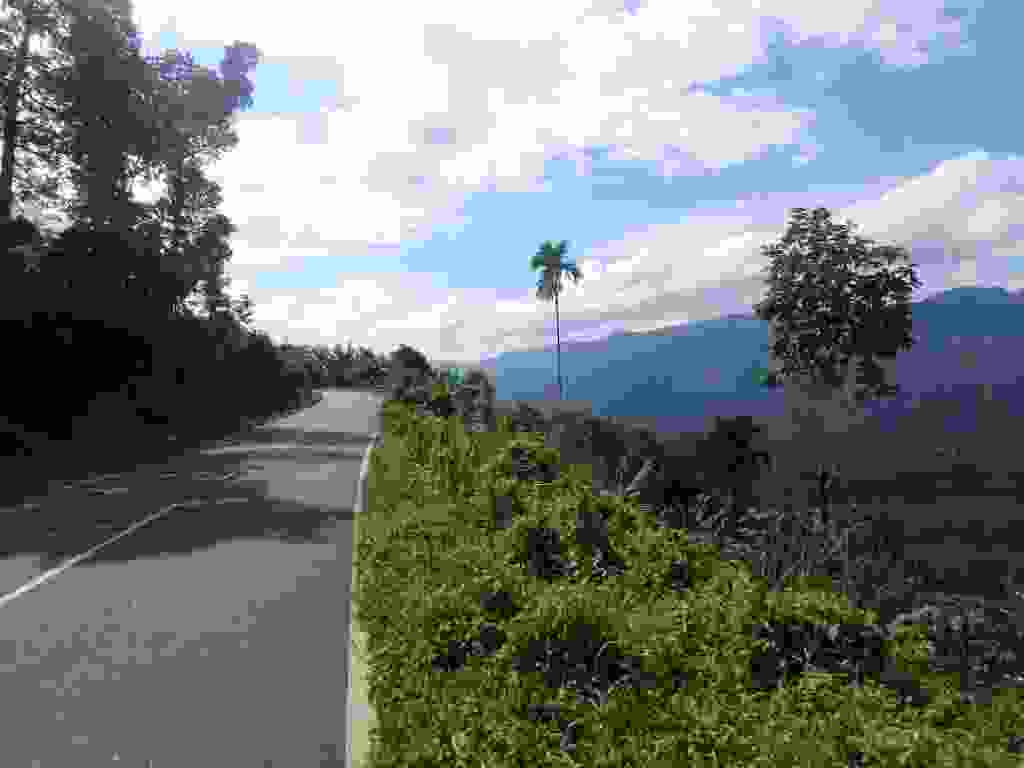
\includegraphics[width=\mywidth]{../wp-content/uploads/2015/11/wpid-oi0002802-1024x768.jpg} } 
 \newline
 La seule nuit de camping en Inde pour le moment : le temps de monter la tente j'avais plein de petites sangsues collées aux pieds, sympa ! \newline
 \newline
\centerline{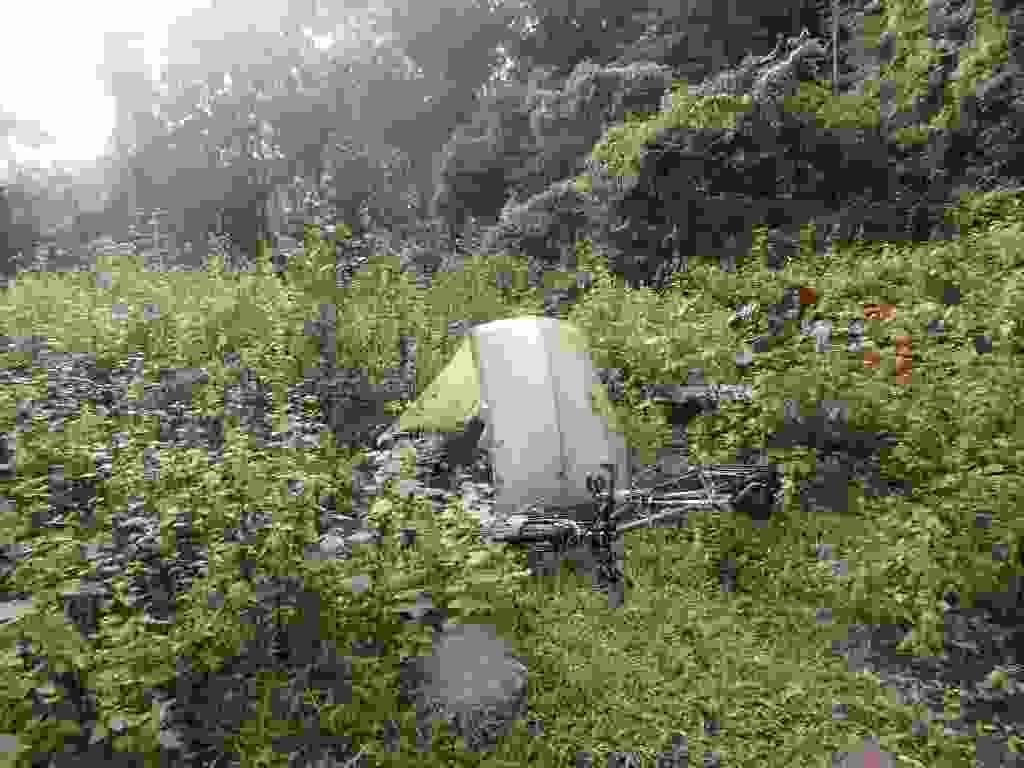
\includegraphics[width=\mywidth]{../wp-content/uploads/2015/11/wpid-oi0002623-1024x768.jpg} } 
 \newline
 Je repasse là où j'étais hébergé avec le groupe de français, le manager avait contacté un reporter d'un journal local pour faire une interview sur le voyage. Pas évident vu qu'il ne parlait pas anglais… \newline
 \newline
\centerline{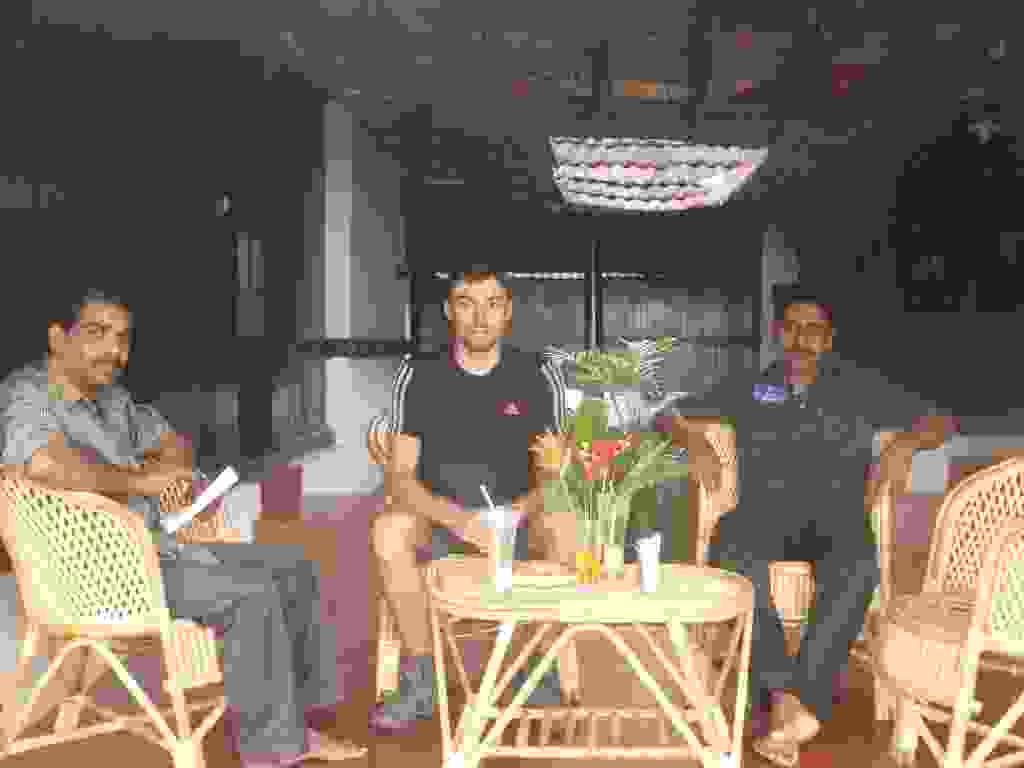
\includegraphics[width=\mywidth]{../wp-content/uploads/2015/11/wpid-oi000315-1024x768.jpg} } 
 \newline
 Puis je roule vers le sud et la ville d'Alleppey \newline
 \newline
\centerline{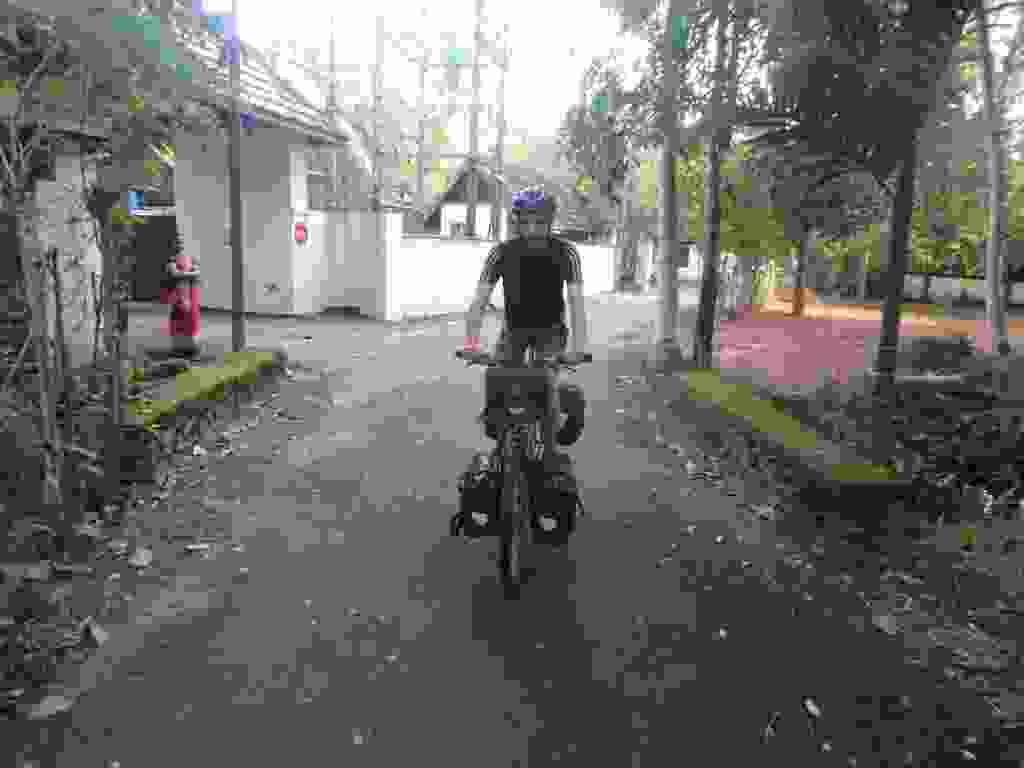
\includegraphics[width=\mywidth]{../wp-content/uploads/2015/11/wpid-oi000321-1024x768.jpg} } 
 \newline
 Beau coucher de soleil en arrivant \newline
 \newline
\centerline{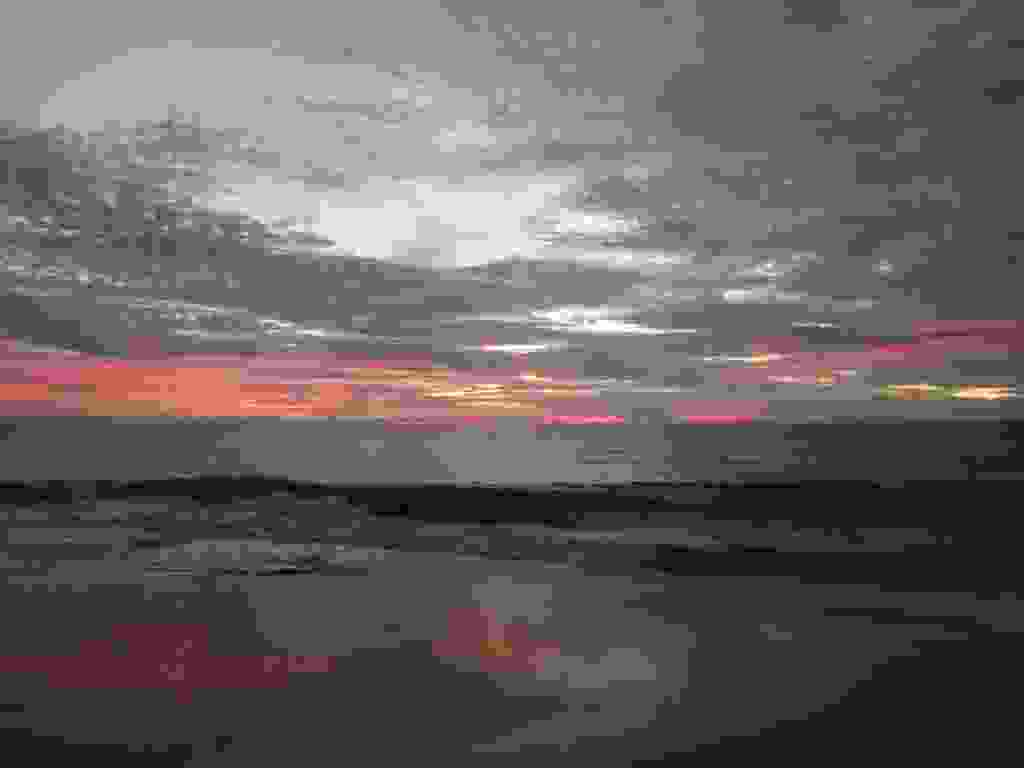
\includegraphics[width=\mywidth]{../wp-content/uploads/2015/11/wpid-oi000324-1024x768.jpg} } 
 \newline
 \newline
\centerline{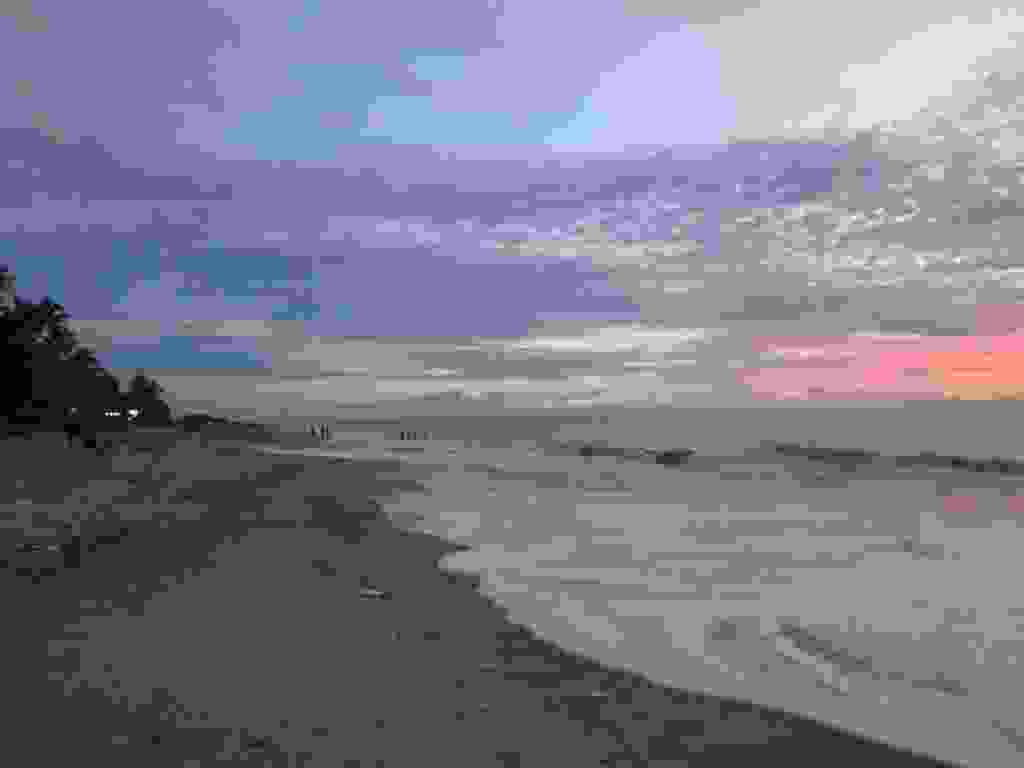
\includegraphics[width=\mywidth]{../wp-content/uploads/2015/11/wpid-oi000326-1024x768.jpg} } 
 \newline
 Je prends des petites routes le long de la côte, j'observe le retour des bateaux de pêche sur une plage \newline
 \newline
\centerline{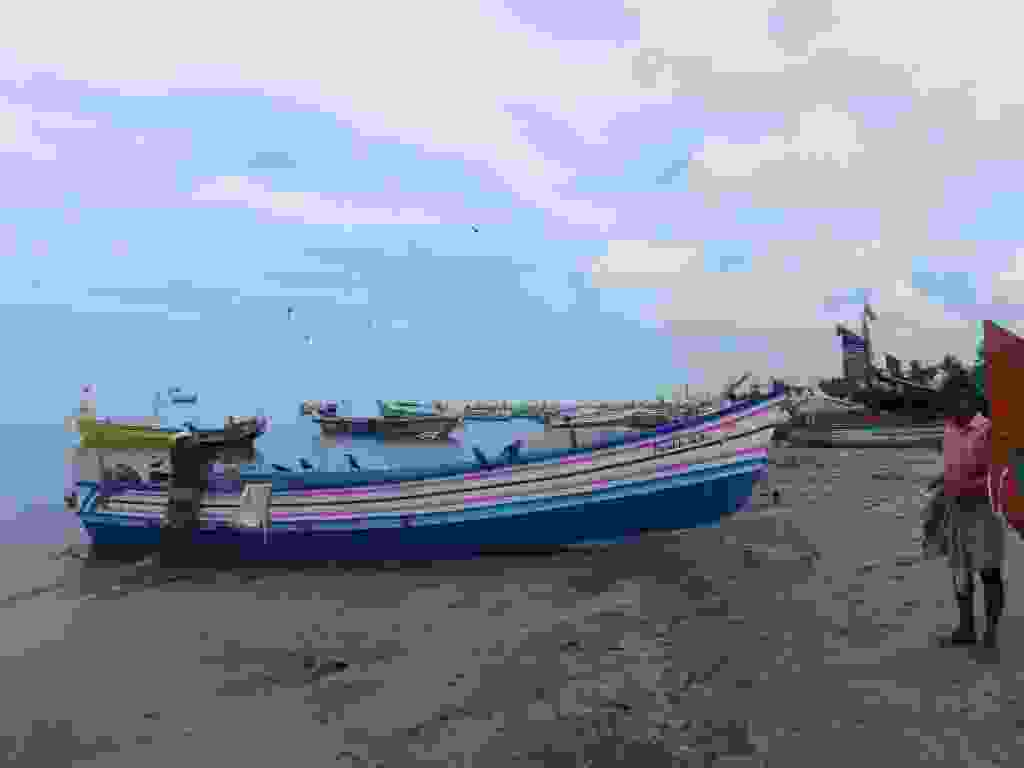
\includegraphics[width=\mywidth]{../wp-content/uploads/2015/11/wpid-oi000334-1024x768.jpg} } 
 \newline
 \newline
\centerline{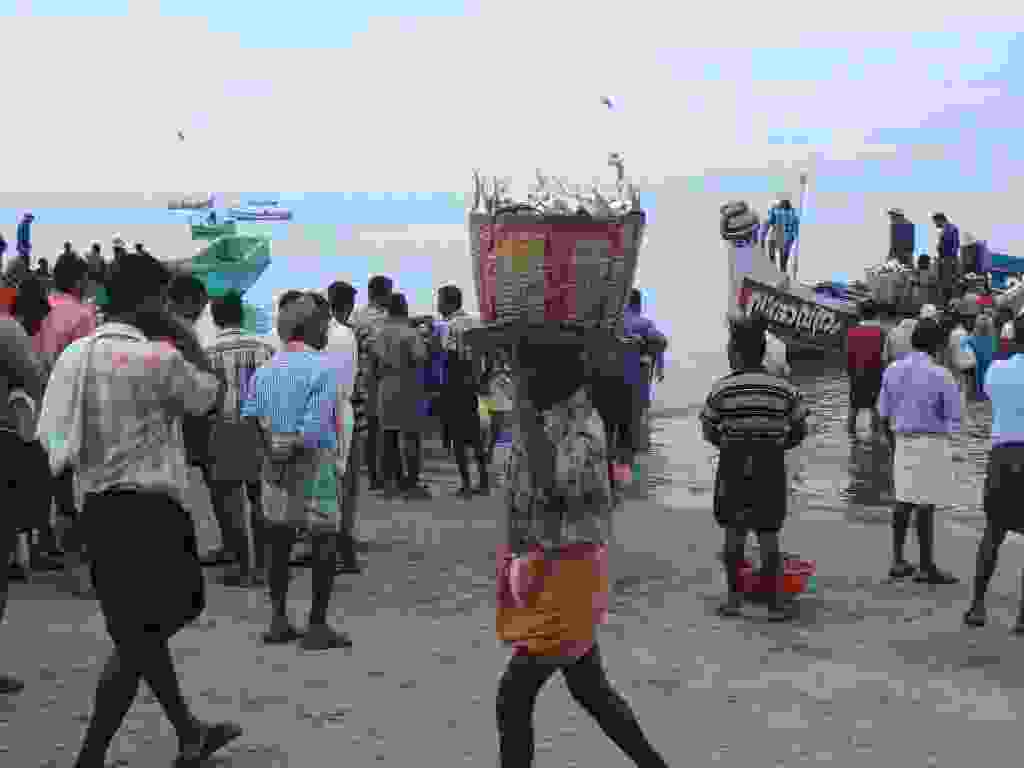
\includegraphics[width=\mywidth]{../wp-content/uploads/2015/11/wpid-oi000333-1024x768.jpg} } 
 \newline
 \newline
\centerline{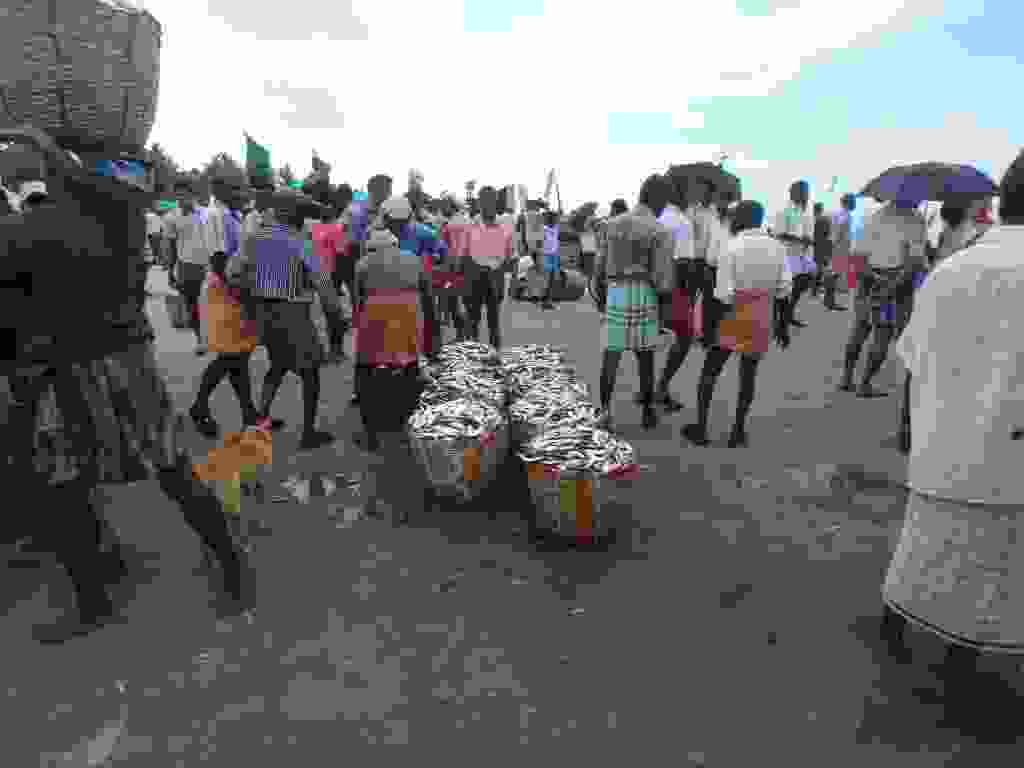
\includegraphics[width=\mywidth]{../wp-content/uploads/2015/11/wpid-oi000336-1024x768.jpg} } 
 \newline
 Dans un village, des gens en train de jouer aux billes \newline
 \newline
\centerline{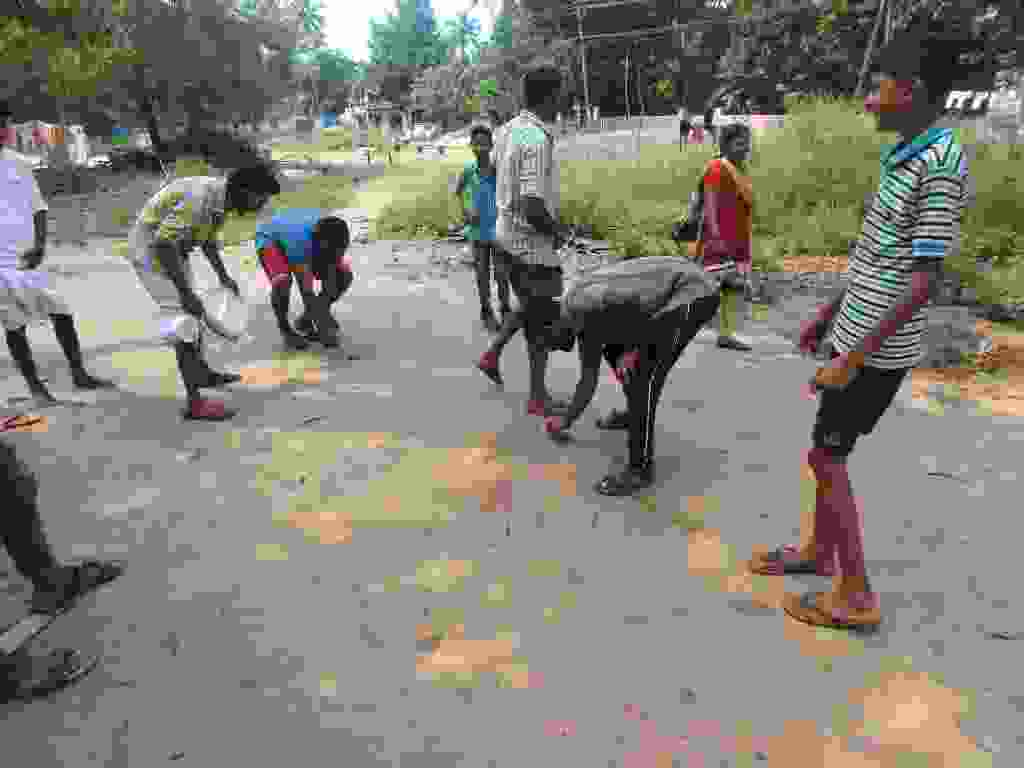
\includegraphics[width=\mywidth]{../wp-content/uploads/2015/11/wpid-oi000338-1024x768.jpg} } 
 \newline
 \newline
\centerline{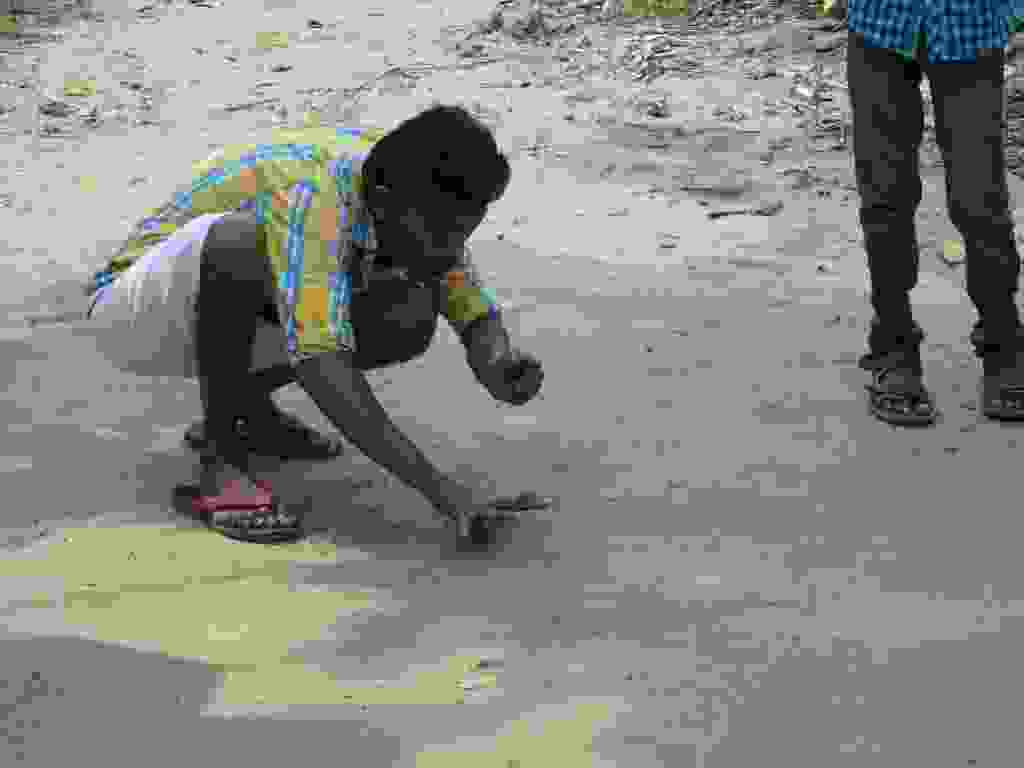
\includegraphics[width=\mywidth]{../wp-content/uploads/2015/11/wpid-oi000339-1024x768.jpg} } 
 \newline
 Petit détour pour visiter le temple d'Ambalapuzha \newline
 \newline
\centerline{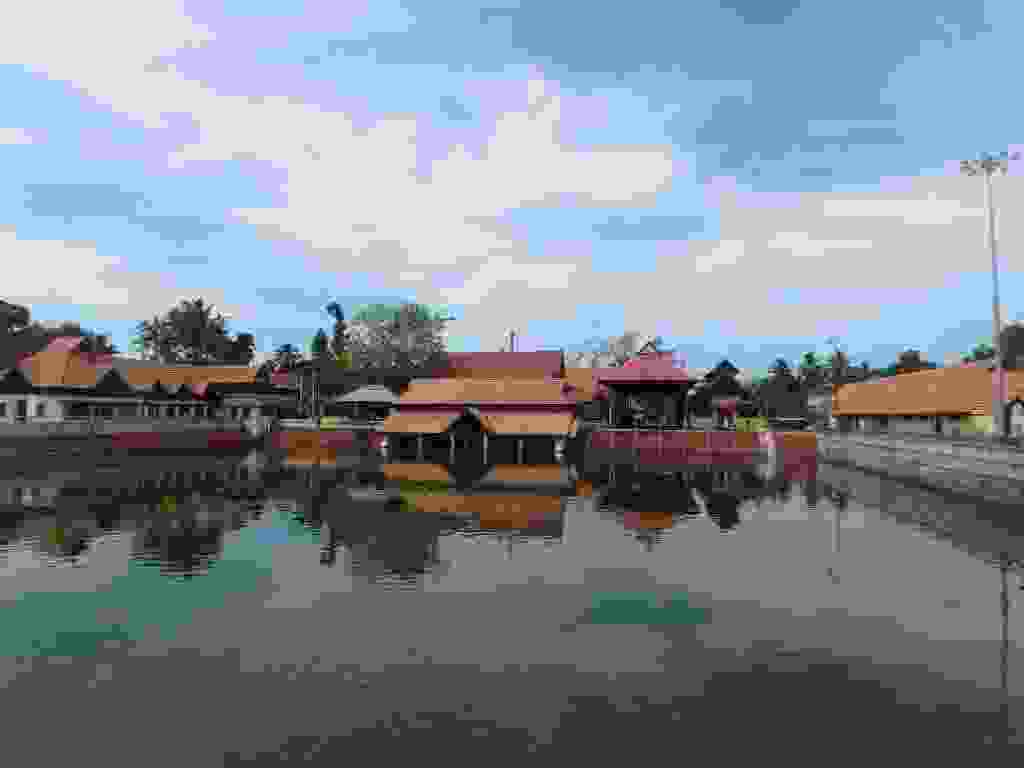
\includegraphics[width=\mywidth]{../wp-content/uploads/2015/11/wpid-oi000346-1024x768.jpg} } 
 \newline
 \newline
\centerline{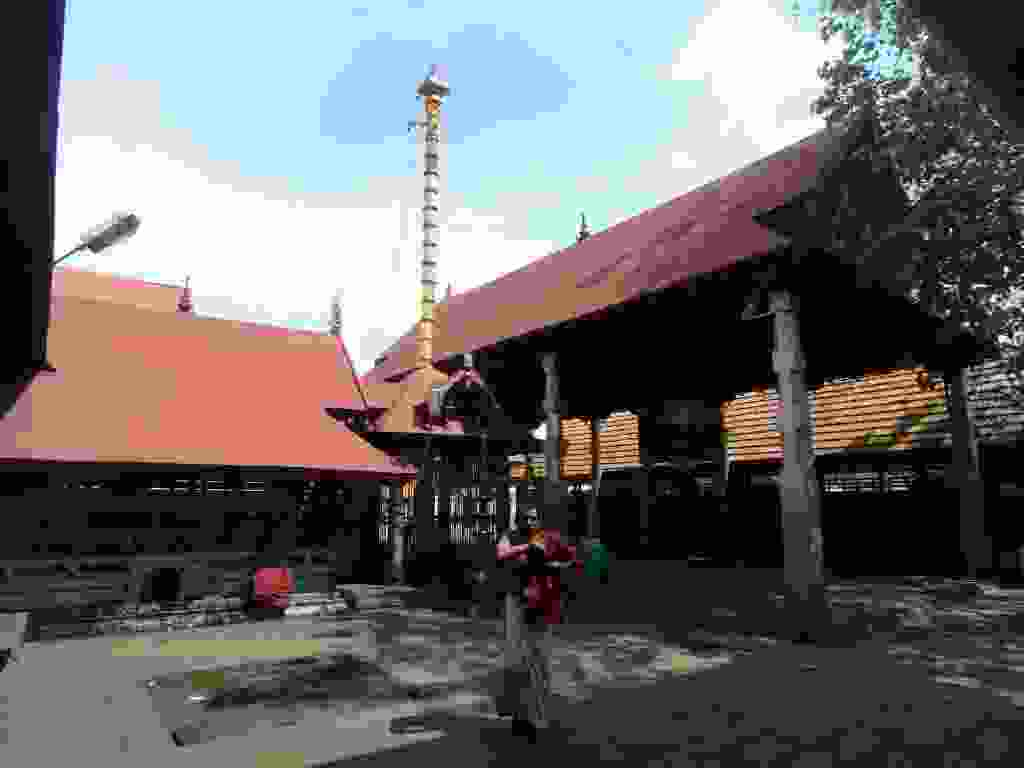
\includegraphics[width=\mywidth]{../wp-content/uploads/2015/11/wpid-oi000342-1024x768.jpg} } 
 \newline
 \newline
\centerline{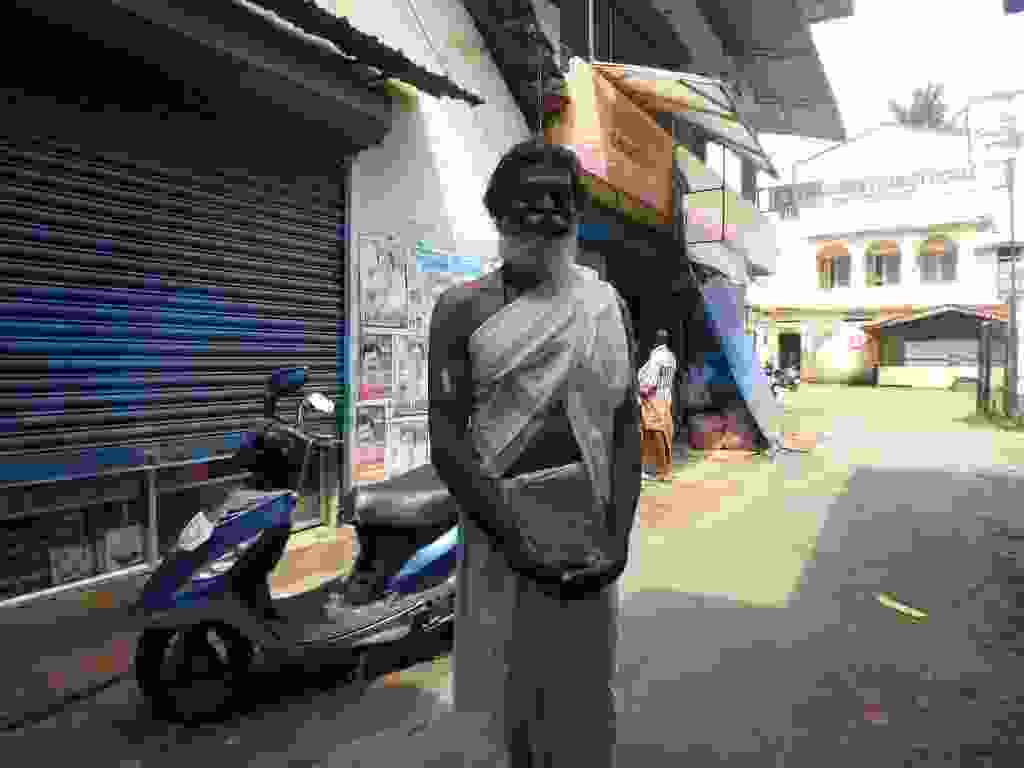
\includegraphics[width=\mywidth]{../wp-content/uploads/2015/11/wpid-oi000347-1024x768.jpg} } 
 \newline
 \newline
\centerline{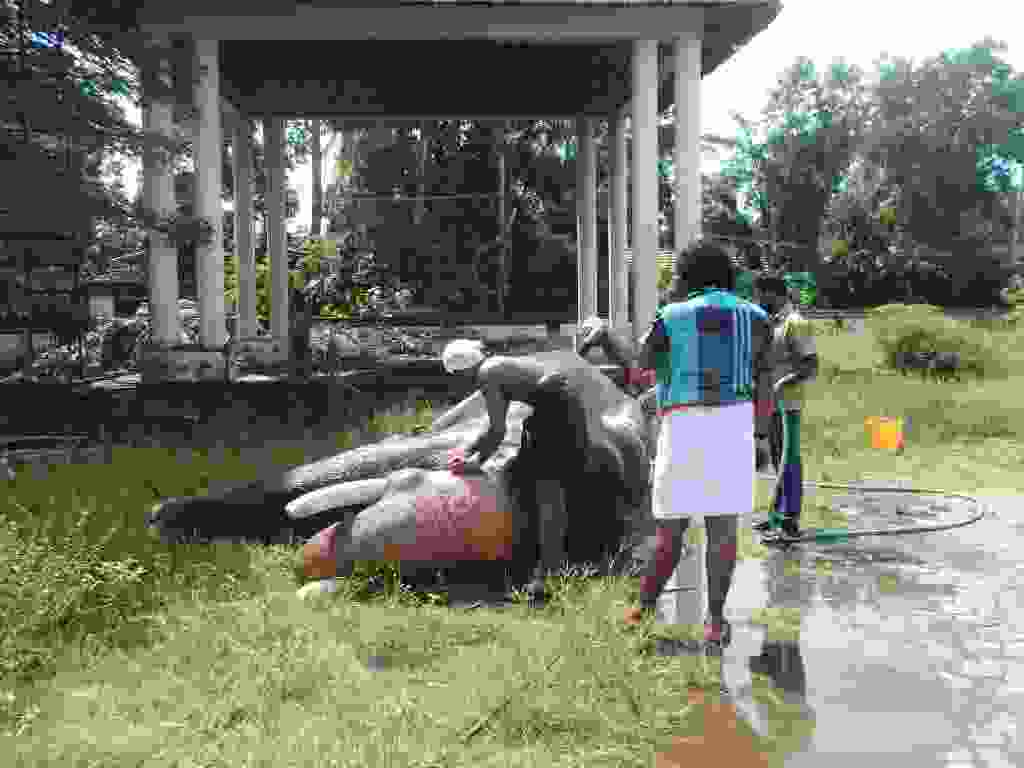
\includegraphics[width=\mywidth]{../wp-content/uploads/2015/11/wpid-oi000344-1024x768.jpg} } 
 \newline
 Palais de Krishnapuram, belle peinture murale. Également une exposition de sculptures mais pas d'électricité pendant la visite, on ne voyait rien \newline
 \newline
\centerline{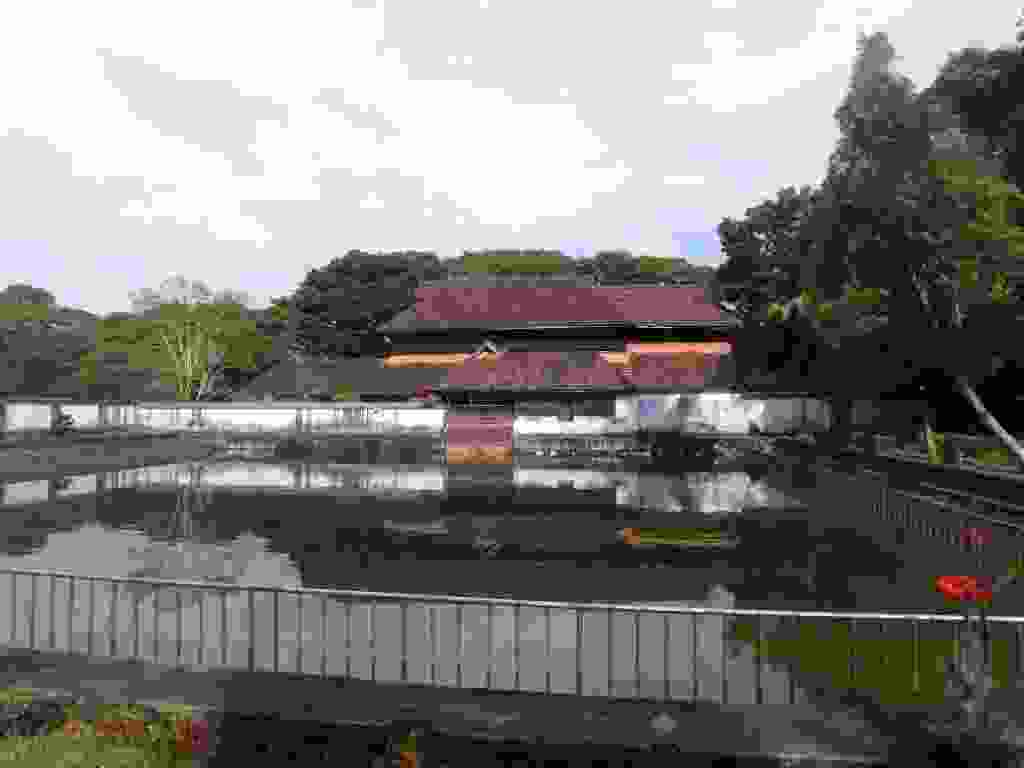
\includegraphics[width=\mywidth]{../wp-content/uploads/2015/11/wpid-oi000359-1024x768.jpg} } 
 \newline
 \newline
\centerline{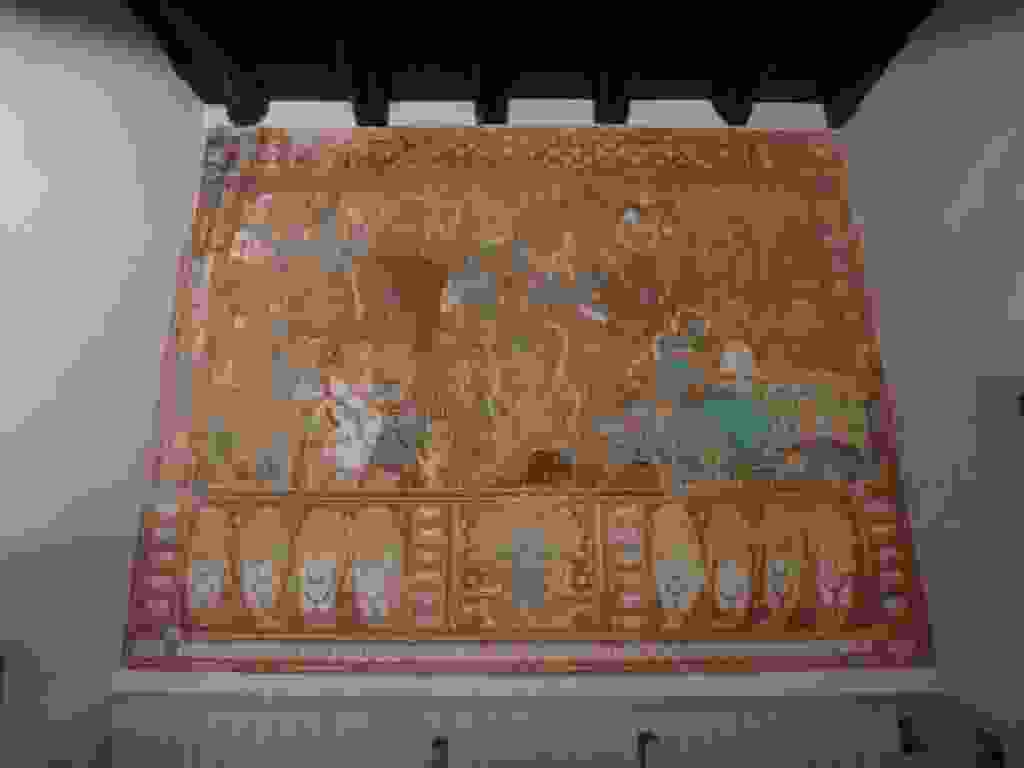
\includegraphics[width=\mywidth]{../wp-content/uploads/2015/11/wpid-oi000351-1024x768.jpg} } 
 \newline
 J'arrive ensuite à Varkala par un petit chemin au bord de la mer \newline
 \newline
\centerline{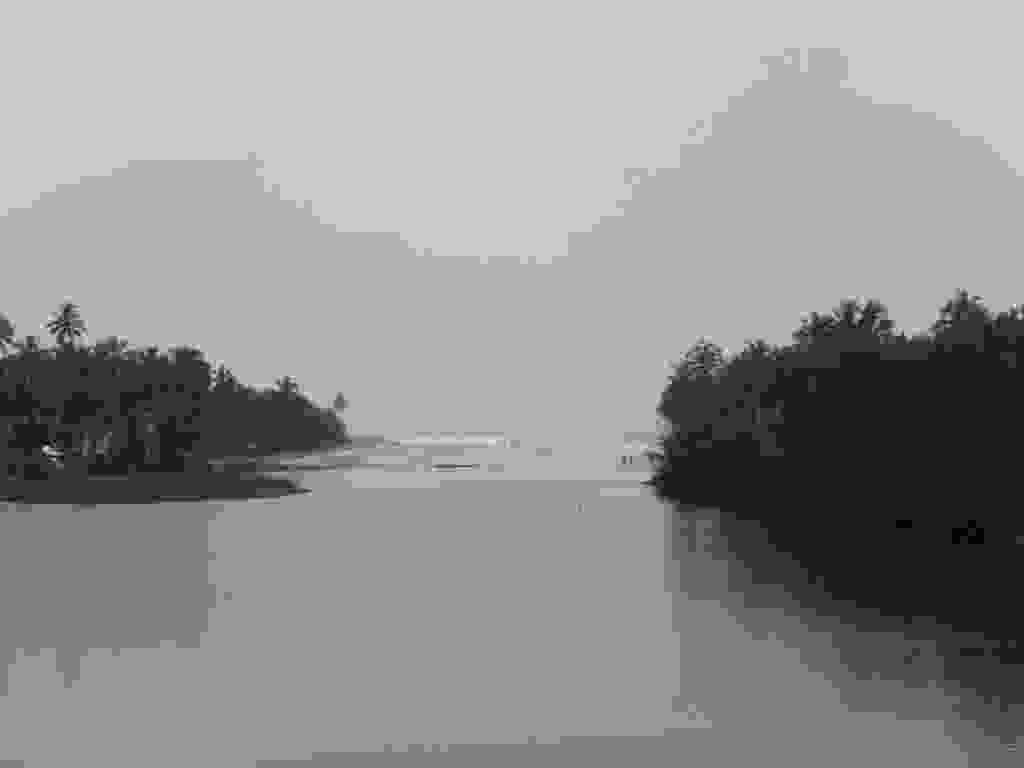
\includegraphics[width=\mywidth]{../wp-content/uploads/2015/11/wpid-oi000368-1024x768.jpg} } 
 \newline
 \newline
\centerline{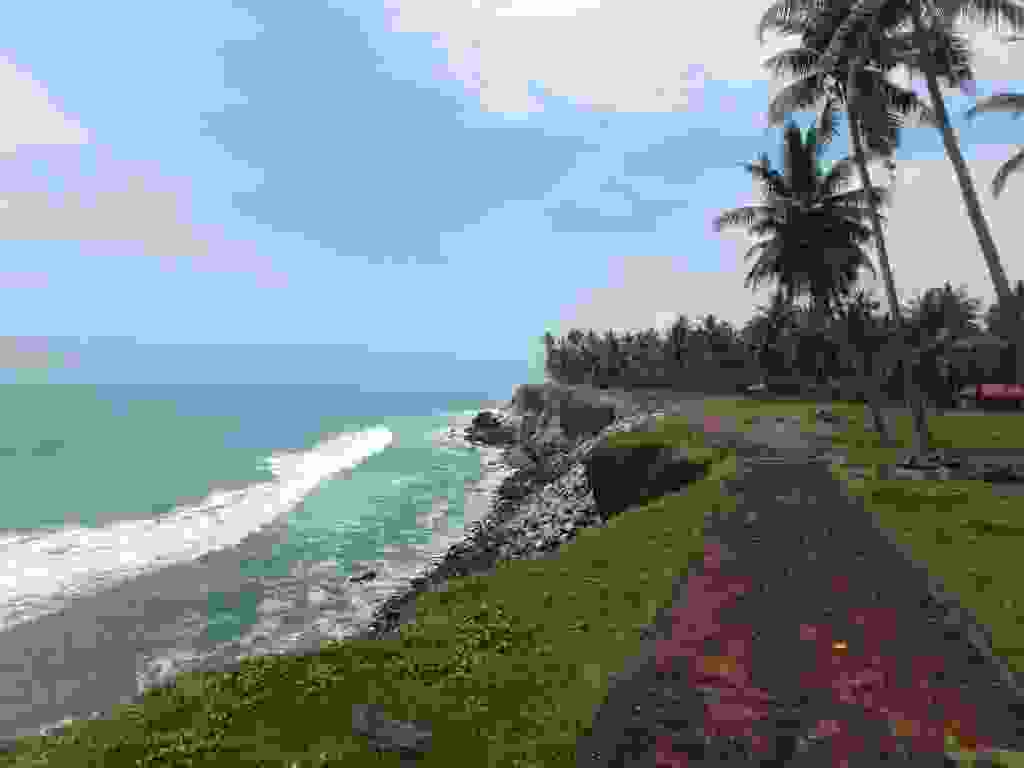
\includegraphics[width=\mywidth]{../wp-content/uploads/2015/11/wpid-oi000370-1024x768.jpg} } 
 \newline
 \newline
\centerline{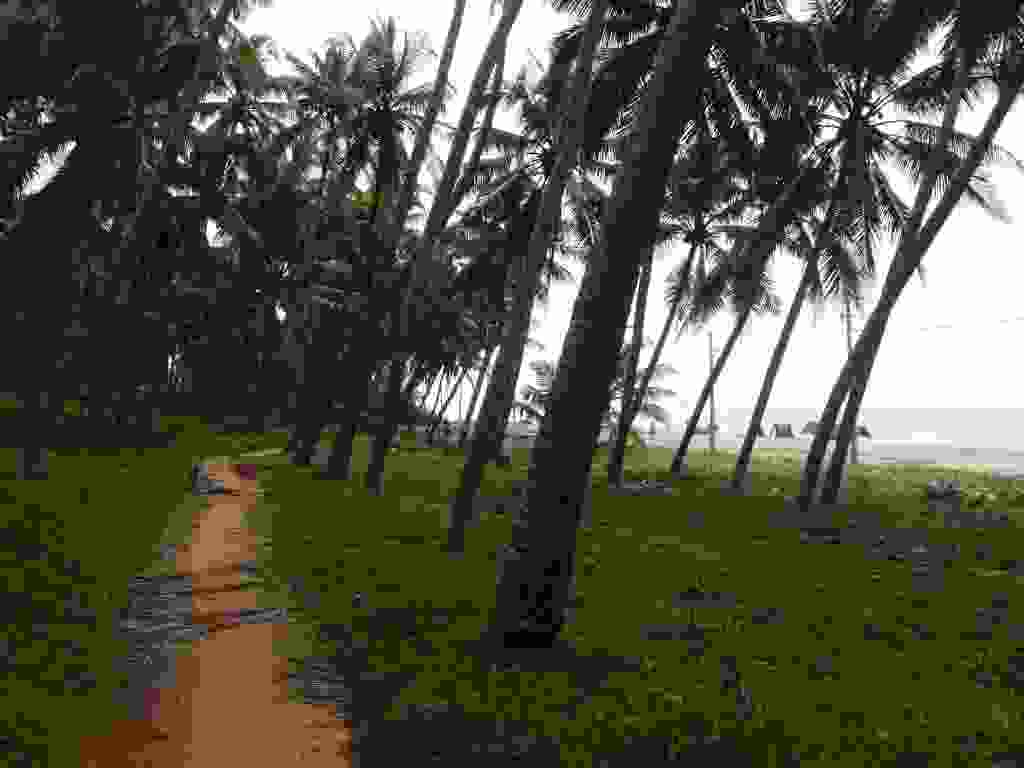
\includegraphics[width=\mywidth]{../wp-content/uploads/2015/11/PB090709-1024x768.jpg} } 
 \newline
 Varkala est une célèbre destination touristique pour les occidentaux, beaucoup d'endroits pour faire des massages ayurvédiques ou du yoga. \newline
 \newline
\centerline{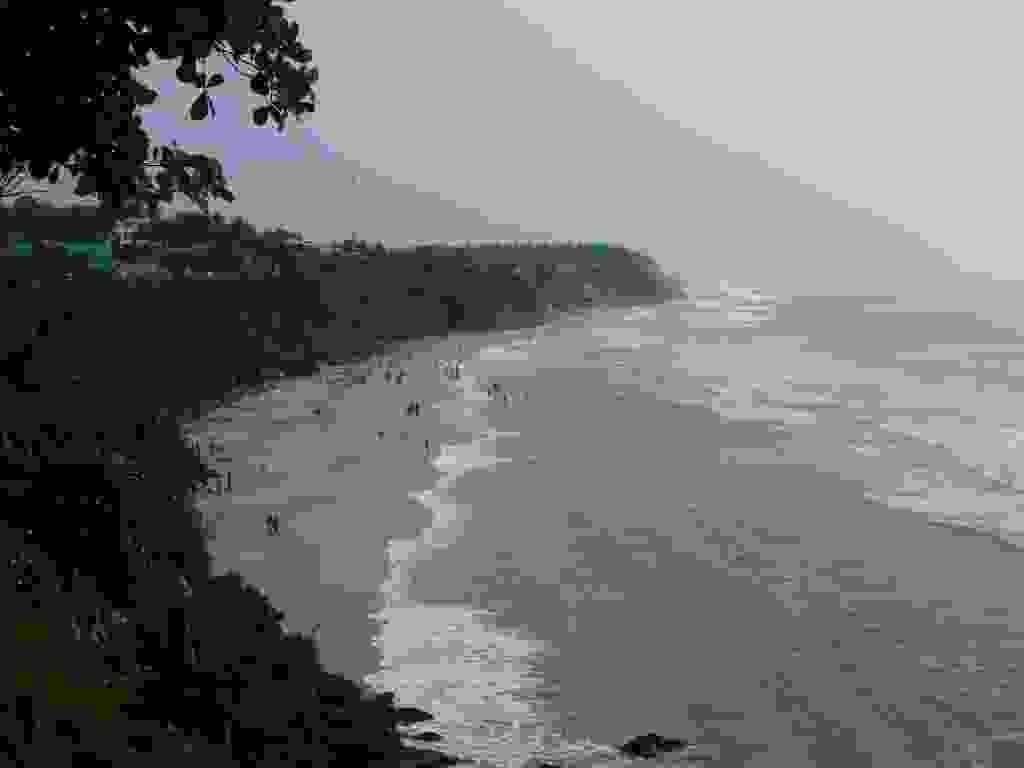
\includegraphics[width=\mywidth]{../wp-content/uploads/2015/11/wpid-oi000373-1024x768.jpg} } 
 \newline
 Le temple Shree Janardhana Swamy dans le village \newline
 \newline
\centerline{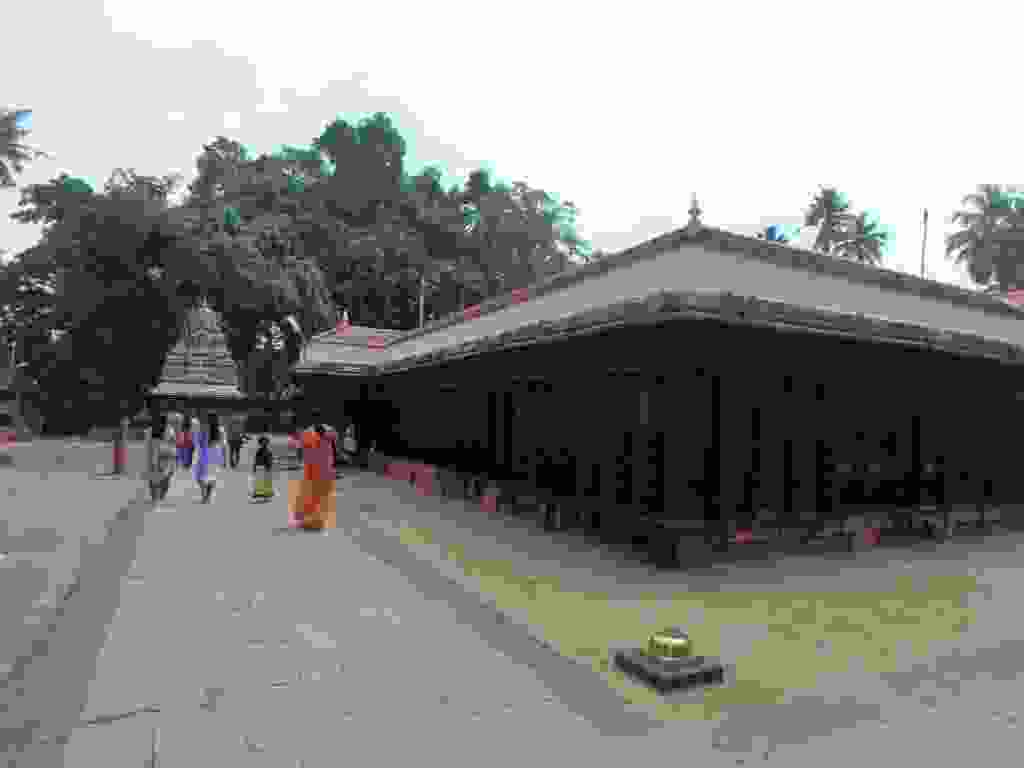
\includegraphics[width=\mywidth]{../wp-content/uploads/2015/11/PB080698-1024x768.jpg} } 
 \newline
 \newline
\centerline{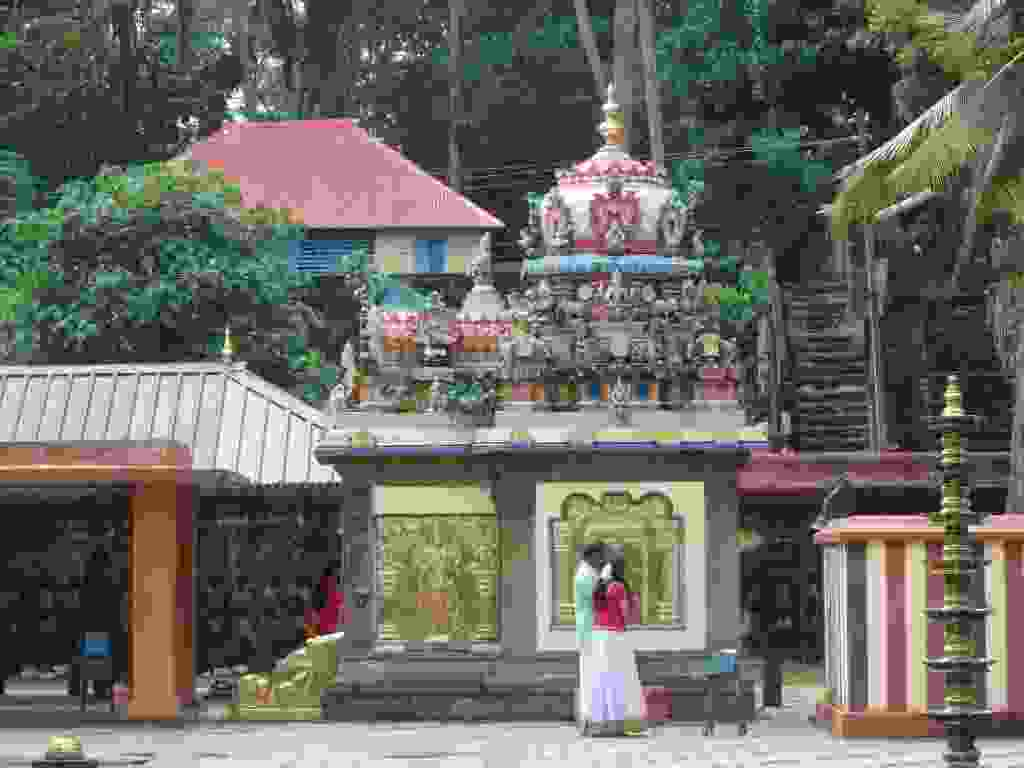
\includegraphics[width=\mywidth]{../wp-content/uploads/2015/11/wpid-oi000379-1024x768.jpg} } 
 \newline
 Je passe ensuite à Trivandrum la capitale du Kerala \newline
 Le temple Sri Padmanabhaswamy, seul les hindous peuvent entrer en respectant la tenue réglementaire \newline
 \newline
\centerline{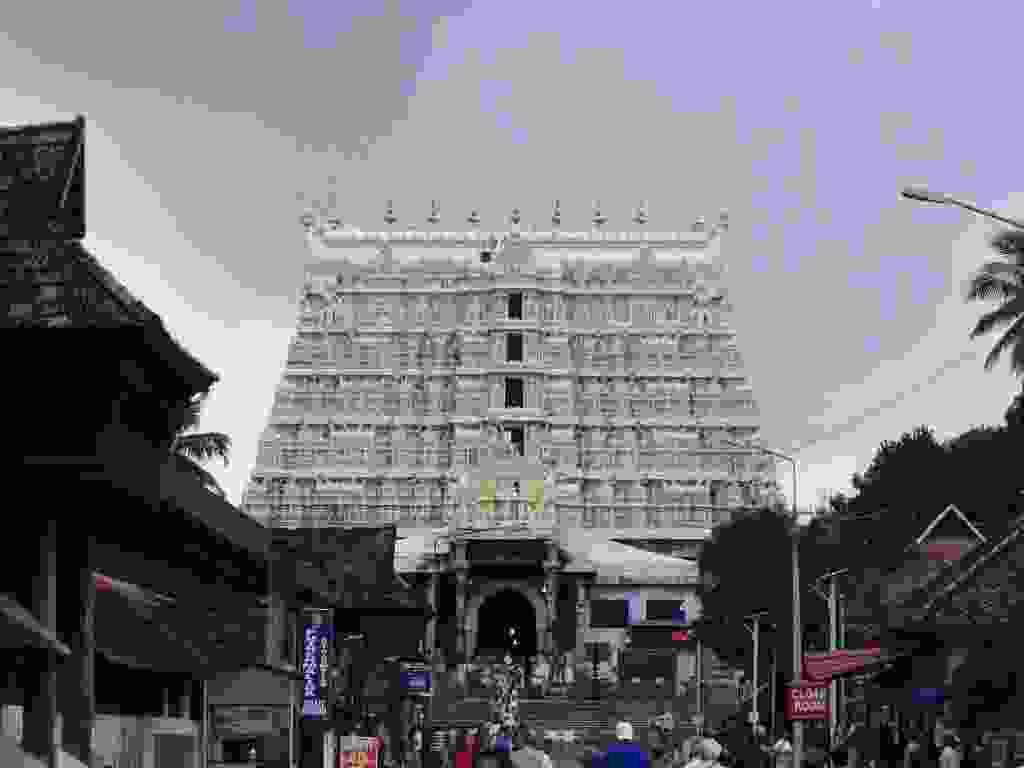
\includegraphics[width=\mywidth]{../wp-content/uploads/2015/11/PB090728-1024x768.jpg} } 
 \newline
 \newline
\centerline{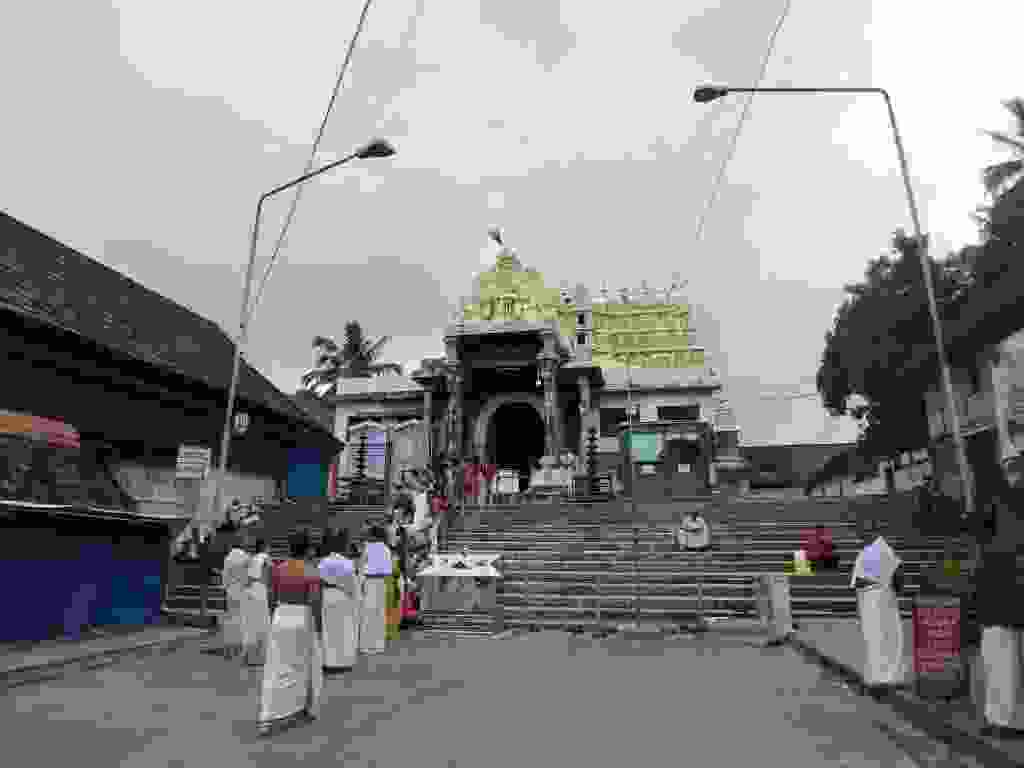
\includegraphics[width=\mywidth]{../wp-content/uploads/2015/11/PB090726-1024x768.jpg} } 
 \newline
 Musée Napier \newline
 \newline
\centerline{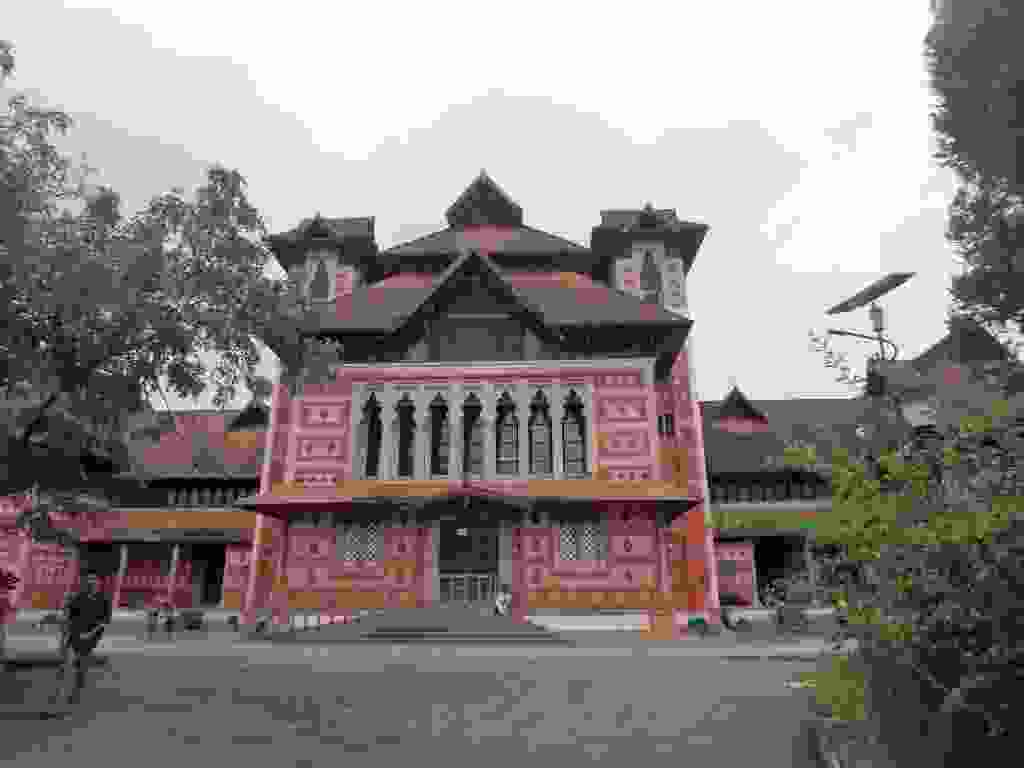
\includegraphics[width=\mywidth]{../wp-content/uploads/2015/11/PB090721-1024x768.jpg} } 
 \newline
 Dernière étape dans le Kerala : Kovalam, dans le même esprit que Varkala avec plus de touristes indiens peut être \newline
 \newline
\centerline{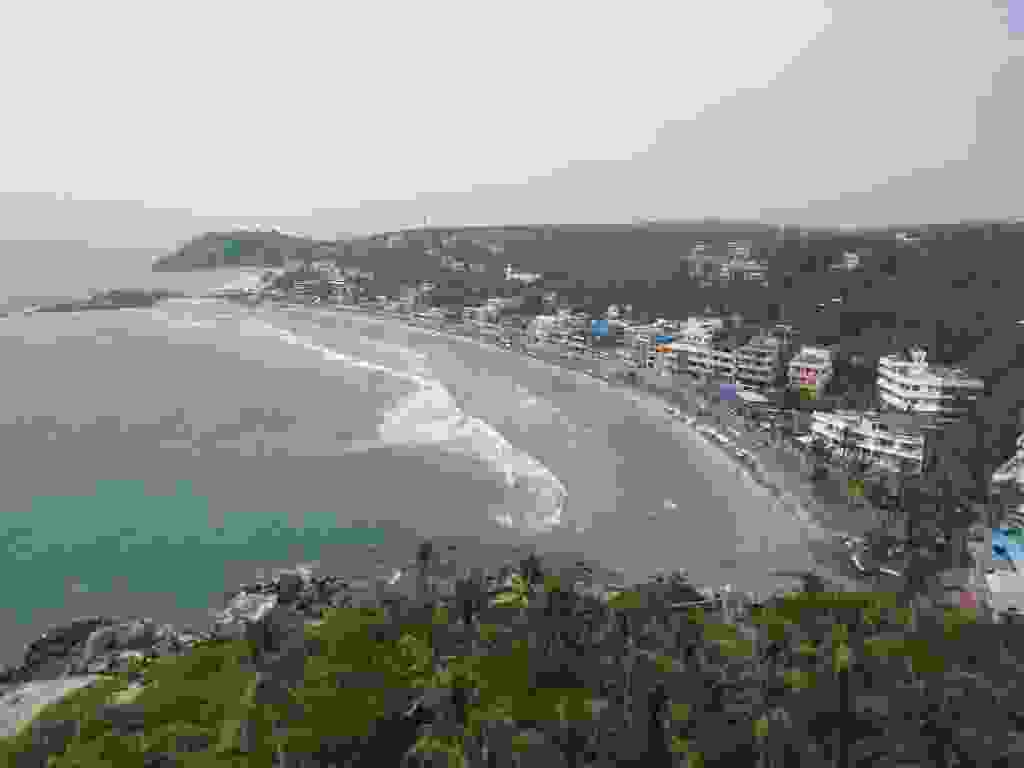
\includegraphics[width=\mywidth]{../wp-content/uploads/2015/11/PB100740-1024x768.jpg} } 
 \newline
 \newline
\centerline{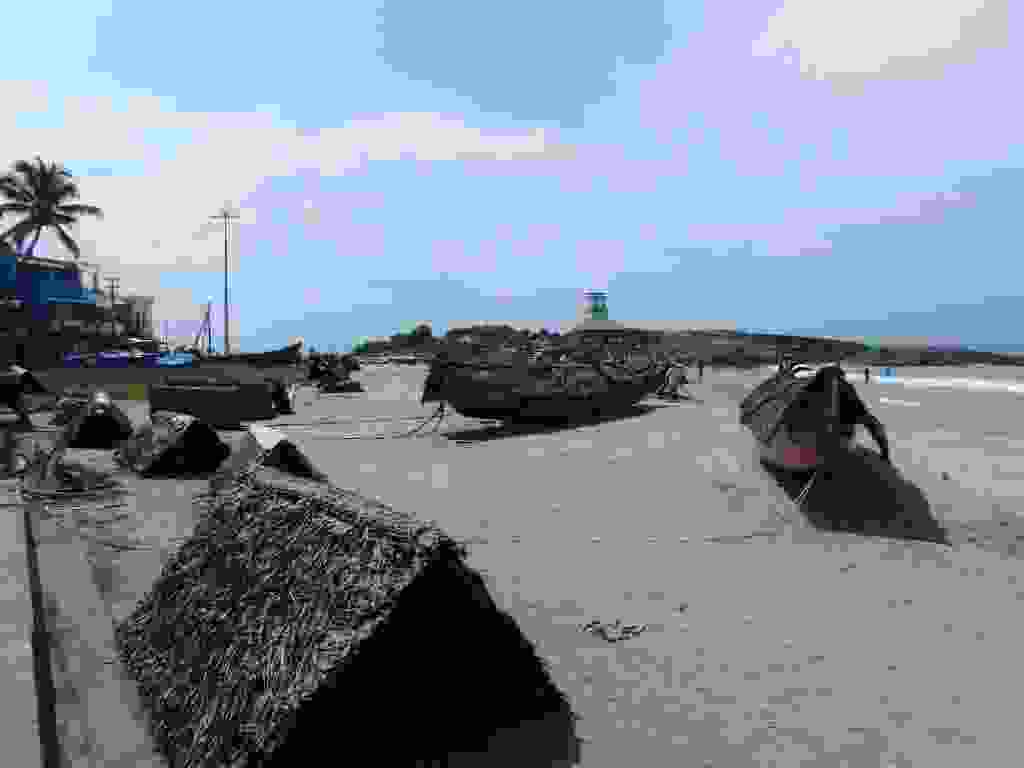
\includegraphics[width=\mywidth]{../wp-content/uploads/2015/11/PB100733-1024x768.jpg} } 
 \newline
 \newline
\centerline{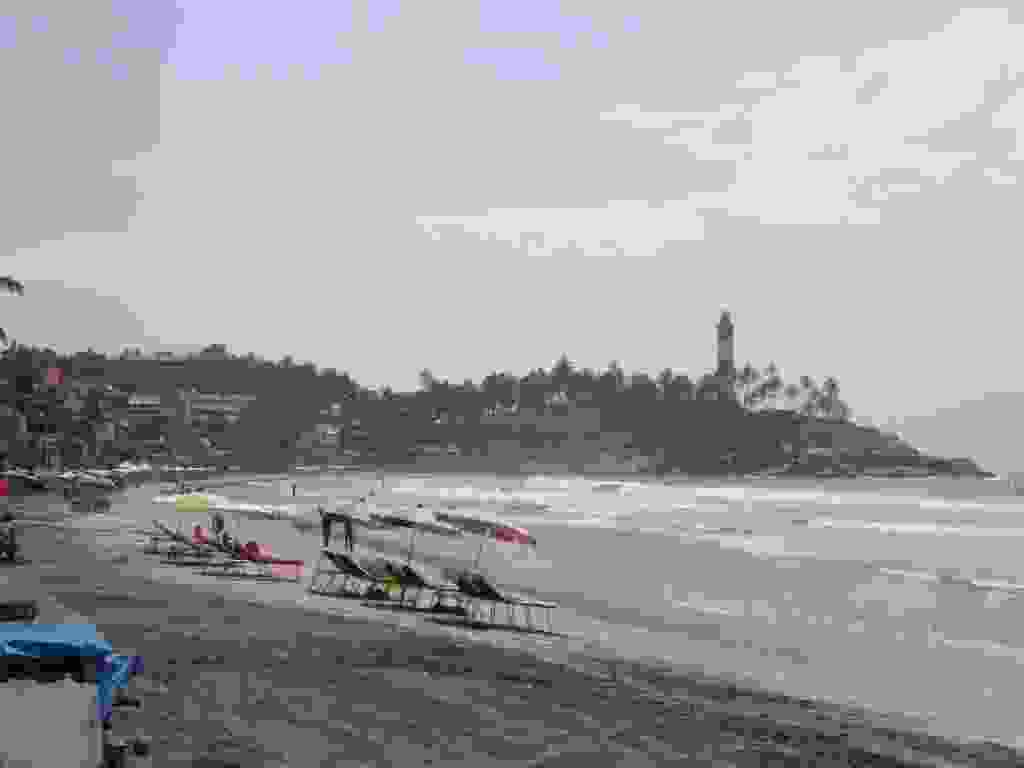
\includegraphics[width=\mywidth]{../wp-content/uploads/2015/11/PB100735-1024x768.jpg} } 
 \newline
 \newline
\centerline{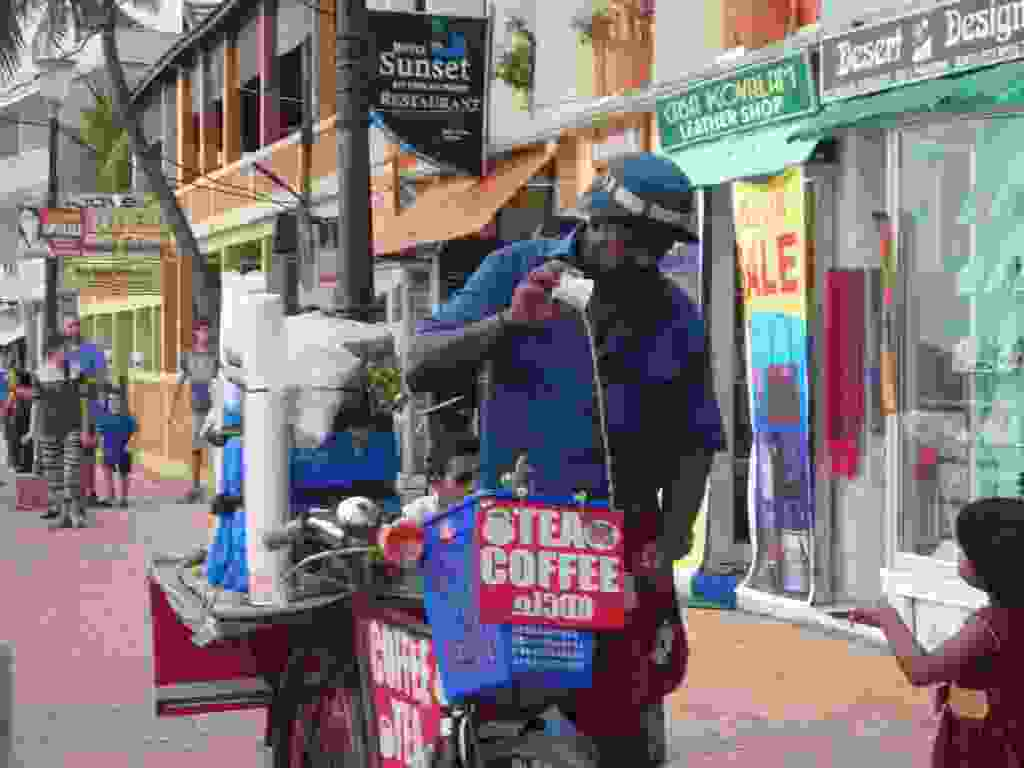
\includegraphics[width=\mywidth]{../wp-content/uploads/2015/11/PB100746-1024x768.jpg} } 
 \newline
 En Inde, difficile de trouver de l'alcool hors des lieux touristiques : seulement dans quelques endroits autorisés et à certaines heures \newline
 \newline
\centerline{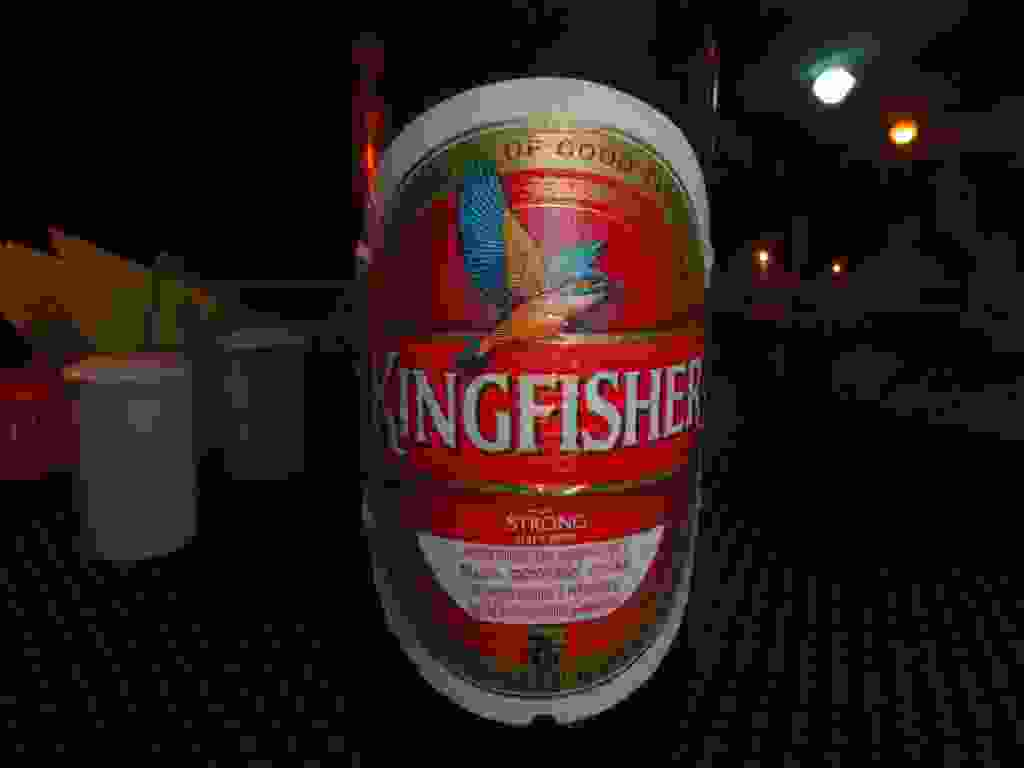
\includegraphics[width=\mywidth]{../wp-content/uploads/2015/11/PB080705-1024x768.jpg} } 
 \newline
 Côté cuisine, Masala Dosa : crêpe remplie de légumes \newline
 \newline
\centerline{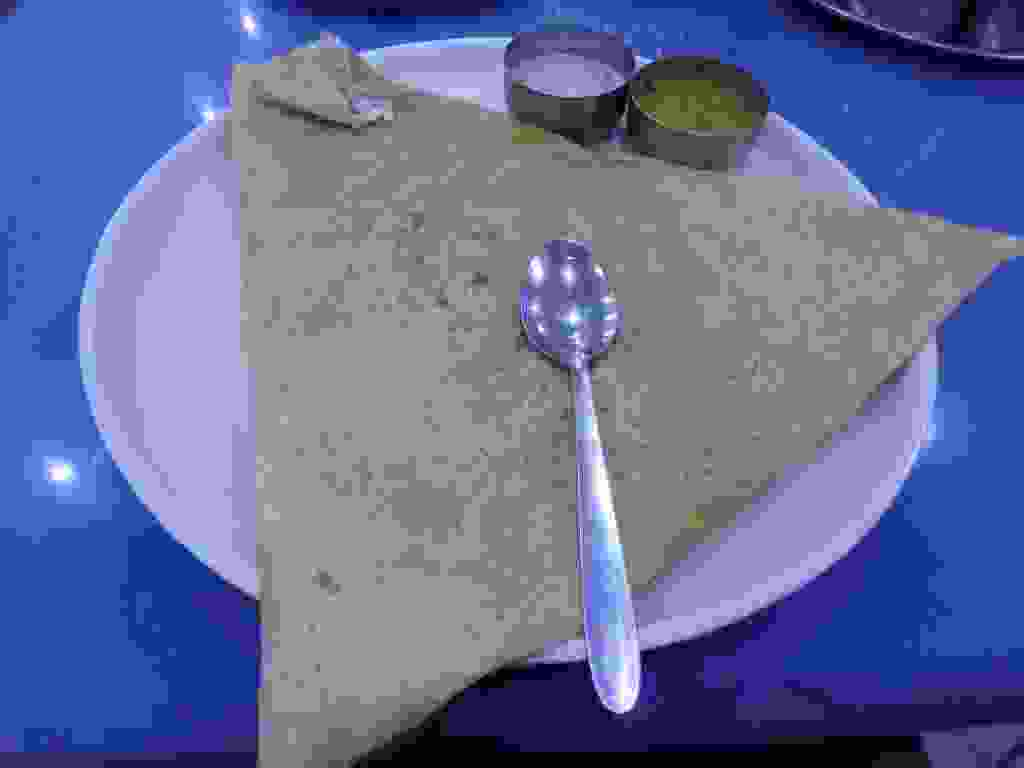
\includegraphics[width=\mywidth]{../wp-content/uploads/2015/11/wpid-oi000363-1024x768.jpg} } 
 \newline

\newpage
 
